\documentclass[11pt]{article}

\usepackage[T1]{fontenc}
\usepackage[utf8]{inputenc}
\usepackage[french]{babel}
\usepackage[a4paper,margin=1in]{geometry}
\usepackage{amsmath,amssymb,amsthm,mathtools}
\usepackage{bm}
\usepackage{graphicx}
\usepackage{booktabs}
\usepackage{float}
\usepackage{enumitem}
\usepackage[font=small,labelfont=bf]{caption}
\usepackage[colorlinks=true,linkcolor=blue,citecolor=blue,urlcolor=blue]{hyperref}

\graphicspath{{figures/}}

\newtheorem{proposition}{Proposition}[section]
\newtheorem{lemma}[proposition]{Lemme}
\theoremstyle{definition}
\newtheorem{definition}[proposition]{Définition}
\theoremstyle{remark}
\newtheorem{remark}[proposition]{Remarque}

\newcommand{\R}{\mathbb{R}}
\newcommand{\E}{\mathbb{E}}
\newcommand{\Neff}{N_{\mathrm{eff}}}
\newcommand{\Nth}{N_{\mathrm{th}}}
\newcommand{\hopt}{h_{\mathrm{opt}}}
\newcommand{\hmnt}{h_{\mathrm{MNT}}}
\newcommand{\T}{\top}

\title{\textbf{Filtrage particulaire régularisé pour la navigation\\ par corrélation de terrain}}
\author{Mohamed Benloughmari \and Fatimetou Narjah}
\date{Filtrage bayésien et navigation --- TP4, ENSTA, 2026}

\begin{document}
\maketitle

\begin{abstract}
On estime la position et la vitesse d'un avion à partir des seules mesures d'un
radio-altimètre, recalées sur un modèle numérique de terrain. La fonction de mesure
est une table de relief, fortement non linéaire, et l'incertitude initiale est de
plusieurs kilomètres : la loi a posteriori est multimodale et le filtrage de Kalman ne
s'applique pas. Nous présentons le filtre particulaire SIR, expliquons sa
dégénérescence, puis le filtre particulaire régularisé (RPF), dans lequel la
redistribution des particules est lissée par un noyau. Sur le scénario du TP
($N=5000$ particules, noyau gaussien), le filtre converge dans les $50$ réalisations
Monte-Carlo effectuées, avec une erreur horizontale médiane de $86$~m en seconde moitié de
vol pour une incertitude initiale de $3$~km. Une étude de sensibilité montre que la
régularisation est indispensable ici (le filtre SIR diverge dans $86\,\%$ des cas) mais
qu'elle doit rester modérée : avec le pas « optimal » non réduit, le filtre diverge
systématiquement.
\end{abstract}

\section{Introduction}

La navigation par corrélation de terrain recale une centrale inertielle, qui dérive,
en comparant la hauteur au-dessus du sol mesurée par un radio-altimètre à une carte
de relief embarquée. Le problème est difficile parce qu'une mesure scalaire ne
désigne pas un point de la carte mais toute une ligne de niveau : c'est la suite des
mesures le long du vol qui lève peu à peu l'ambiguïté.

Ce rapport répond à cinq questions : pourquoi un filtre particulaire
(section~\ref{sec:modele}) ; comment fonctionne le filtre SIR et pourquoi il dégénère
(section~\ref{sec:sir}) ; ce qu'apporte la régularisation (section~\ref{sec:rpf}) ;
si le filtre converge sur le scénario du TP (section~\ref{sec:resultats}) ; et
quelle est sa sensibilité aux paramètres (section~\ref{sec:sensibilite}). Le filtre
étant aléatoire, toutes les comparaisons reposent sur $50$ réalisations Monte-Carlo
par configuration, avec les mêmes graines d'une configuration à l'autre.

\section{Modèle et difficulté du problème}\label{sec:modele}

\subsection{Modèle d'état}

L'état est $X_k=(x_k,y_k,z_k,\dot x_k,\dot y_k,\dot z_k)^\T\in\R^6$. L'avion suit un
mouvement rectiligne uniforme et l'on mesure sa hauteur au-dessus du sol :
\begin{equation}\label{eq:modele}
\begin{cases}
X_k=\Phi X_{k-1}+\eta_k, & \Phi=\begin{pmatrix} I_3 & \Delta t\,I_3\\ 0 & I_3\end{pmatrix},
\quad \eta_k\sim\mathcal N(0,Q),\\[4pt]
Y_k=z_k-\hmnt(x_k,y_k)+\epsilon_k, & \epsilon_k\sim\mathcal N(0,\sigma^2),
\end{cases}
\end{equation}
où $\hmnt$ est l'altitude du relief donnée par le modèle numérique de terrain (MNT).
La dynamique est linéaire et gaussienne ; toute la difficulté vient de la mesure.
La carte utilisée compte $799\times799$ mailles de $334$~m en $x$ sur $464$~m en $y$,
interpolées bilinéairement, avec la convention d'indexation $\mathrm{MNT}(y,x)$.

\subsection{Pourquoi le filtre de Kalman ne convient pas}

Le filtre de Kalman suppose une mesure linéaire en l'état, ce que $\hmnt$ n'est pas.
Le filtre de Kalman étendu linéarise la mesure autour de l'estimée courante :
\begin{equation}\label{eq:jacobienne}
H_k=\Bigl(-\partial_x\hmnt,\ -\partial_y\hmnt,\ 1,\ 0,\ 0,\ 0\Bigr)\Big|_{\hat X_{k|k-1}} .
\end{equation}
Cette linéarisation n'est valable que si l'erreur de position est petite devant
l'échelle de variation du relief. Or l'incertitude initiale ($3$~km d'écart-type)
couvre une dizaine de mailles dans chaque direction : le gradient calculé à
l'estimée n'a aucune raison de ressembler au gradient au point vrai. De plus, le
filtre étendu propage une seule gaussienne, alors que plusieurs zones éloignées de
la carte peuvent expliquer aussi bien les premières mesures. La loi a posteriori est
donc multimodale, comme le confirme la figure~\ref{fig:carte} à $t=30$~s.

\subsection{Observabilité}

L'expression~\eqref{eq:jacobienne} montre d'où vient l'information. Au-dessus d'un
terrain plat, $\nabla\hmnt=0$ : la mesure ne renseigne que sur $z$, et la position
horizontale n'est pas observable. Elle ne le devient que si le gradient du relief
change de direction le long de la trajectoire, chaque mesure contraignant alors une
direction différente du plan. Les vitesses, qui n'apparaissent pas dans la mesure,
ne sont observables qu'à travers $\Phi$, par l'évolution de la position ; on s'attend
donc à ce qu'elles convergent plus lentement.

Enfin, $z$ et $\hmnt$ n'interviennent que par leur différence. Un déplacement
horizontal qui change le relief de $\delta h$ est exactement compensé par une erreur
d'altitude $\delta h$ : tant que $z$ est mal connu ($500$~m d'écart-type initial), une
mesure isolée n'élimine presque aucune hypothèse de position.

\section{Filtre SIR et dégénérescence}\label{sec:sir}

\subsection{Approximation particulaire et mise à jour des poids}

Le filtre particulaire~\cite{gordon,arulampalam} approche la loi a posteriori par une mesure empirique pondérée,
\[
p(x_k\mid Y_{1:k})\approx\sum_{j=1}^N w_k^j\,\delta_{X_k^j}(x),\qquad
w_k^j\ge0,\quad\sum_j w_k^j=1 .
\]

\begin{proposition}[Mise à jour des poids]\label{prop:poids}
Si les particules sont propagées selon la loi de transition,
$X_k^j\sim p(x_k\mid X_{k-1}^j)$, les poids d'importance vérifient
\begin{equation}\label{eq:poids}
w_k^j\ \propto\ w_{k-1}^j\;p\bigl(Y_k\mid X_k^j\bigr).
\end{equation}
\end{proposition}

\begin{proof}
Par la formule de Bayes et la propriété de Markov, la loi cible de la trajectoire se
factorise en
$p(x_{0:k}\mid Y_{1:k})\propto p(Y_k\mid x_k)\,p(x_k\mid x_{k-1})\,p(x_{0:k-1}\mid Y_{1:k-1})$.
La loi de proposition est
$q(x_{0:k})=p(x_k\mid x_{k-1})\,q(x_{0:k-1})$. Le poids d'importance est le rapport
cible sur proposition : le facteur $p(x_k\mid x_{k-1})$ se simplifie et il reste
$w_k\propto p(Y_k\mid x_k)\,w_{k-1}$.
\end{proof}

Pour le modèle~\eqref{eq:modele}, la vraisemblance est
$p(Y_k\mid X)\propto\exp\bigl(-(Y_k-z+\hmnt(x,y))^2/2\sigma^2\bigr)$. L'état et son incertitude sont estimés par la moyenne et la covariance pondérées
\[
\hat X_k=\sum_j w_k^jX_k^j,\qquad
P_k=\sum_j w_k^j(X_k^j-\hat X_k)(X_k^j-\hat X_k)^\T .
\]

\begin{remark}[Calcul en logarithme]
Au début du vol, l'innovation d'une particule dépasse couramment $1500$~m. Avec
$\sigma=30$~m, sa vraisemblance vaut $\exp(-1250)$, qui est nul en double précision : si
toutes les particules sont dans ce cas, la normalisation donne $0/0$. Nous calculons
donc $\log w$, retranchons son maximum, puis prenons l'exponentielle.
\end{remark}

\subsection{Dégénérescence et taille effective}

La relation~\eqref{eq:poids} multiplie les poids à chaque pas. Leur contraste ne fait
qu'augmenter : on montre que la variance des poids non normalisés croît avec le
temps~\cite{kong}, même si le modèle est exact. Au bout de quelques dizaines de mesures,
une seule particule porte presque tout le poids et les $N-1$ autres ne contribuent
plus à l'estimation. On mesure ce phénomène par la taille effective de l'échantillon.

\begin{definition}
$\displaystyle\Neff=\frac{1}{\sum_{j=1}^N (w_k^j)^2}$.
\end{definition}

\begin{proposition}\label{prop:neff}
On a $1\le\Neff\le N$. La borne supérieure est atteinte si et seulement si les poids
sont uniformes, la borne inférieure si et seulement si un seul poids est non nul.
\end{proposition}

\begin{proof}
Par l'inégalité de Cauchy--Schwarz,
$1=\bigl(\sum_j w^j\cdot1\bigr)^2\le N\sum_j (w^j)^2$, avec égalité si et seulement
si les $w^j$ sont tous égaux, d'où $\Neff\le N$. Par ailleurs $0\le w^j\le1$ donne
$(w^j)^2\le w^j$, donc $\sum_j (w^j)^2\le1$ et $\Neff\ge1$, avec égalité si et
seulement si chaque $w^j$ vaut $0$ ou $1$.
\end{proof}

\subsection{Rééchantillonnage multinomial}

Lorsque $\Neff<\Nth=c\,N$, on tire $N$ indices indépendants $I_1,\dots,I_N$ avec
$\mathbb P(I_i=j)=w^j$, on remplace le nuage par $(X^{I_i})_i$ et l'on remet les poids
à $1/N$. Les particules lourdes sont dupliquées, les légères disparaissent.

\begin{proposition}[Absence de biais]\label{prop:multi}
Soit $n^j$ le nombre de copies de la particule $j$. Alors $\E[n^j]=Nw^j$ et
$\operatorname{Var}(n^j)=Nw^j(1-w^j)$. Pour toute fonction test $\varphi$, conditionnellement
au nuage,
\[
\E\Bigl[\tfrac1N\textstyle\sum_i\varphi(X^{I_i})\Bigr]=\sum_j w^j\varphi(X^j),\qquad
\operatorname{Var}\Bigl[\tfrac1N\textstyle\sum_i\varphi(X^{I_i})\Bigr]
=\frac1N\operatorname{Var}_w(\varphi),
\]
où $\operatorname{Var}_w(\varphi)=\sum_jw^j\varphi(X^j)^2-\bigl(\sum_jw^j\varphi(X^j)\bigr)^2$.
\end{proposition}

\begin{proof}
Le vecteur des $n^j$ suit une loi multinomiale de paramètres $N$ et $(w^j)_j$,
d'où l'espérance et la variance de $n^j$. Les $\varphi(X^{I_i})$
sont indépendants et de même loi, d'espérance $\sum_jw^j\varphi(X^j)$ et de variance
$\operatorname{Var}_w(\varphi)$ ; la moyenne de $N$ tels termes a la variance annoncée.
\end{proof}

Le rééchantillonnage ne biaise donc pas l'estimation mais lui ajoute une variance en
$1/N$. C'est pourquoi on calcule $\hat X_k$ et $P_k$ \emph{avant} de redistribuer, et
pourquoi on ne redistribue que lorsque $\Neff$ passe sous le seuil.

Le défaut de ce schéma est l'appauvrissement : après redistribution, beaucoup de
particules sont des copies exactes. Seul le bruit d'état $\eta_k$ les sépare ensuite.
Si ce bruit est faible --- ici $0{,}5$~m par pas en position pour un nuage large de
plusieurs kilomètres --- le nuage ne peut plus explorer l'espace d'état, et il suffit
qu'aucune copie ne soit proche de l'état vrai pour que le filtre soit perdu.

\section{Régularisation}\label{sec:rpf}

\subsection{Lissage par un noyau}

Le filtre régularisé~\cite{musso} remplace la mesure empirique discrète par une densité,
obtenue par convolution avec un noyau :
\begin{equation}\label{eq:melange}
\hat p_h(x)=\sum_{j=1}^N w^j K_h(x-X^j),\qquad K_h(x)=\frac1{h^d}K\Bigl(\frac xh\Bigr),
\end{equation}
où $K$ est une densité sur $\R^d$ centrée et de second moment fini :
$K\ge0$, $\int K=1$, $\int xK(x)\,dx=0$, $\int\|x\|^2K(x)\,dx<\infty$. Nous utilisons
le noyau gaussien $K(x)=(2\pi)^{-d/2}e^{-\|x\|^2/2}$ et le noyau d'Epanechnikov
$K(x)=\frac{d+2}{2c_d}(1-\|x\|^2)\mathbf 1_{\|x\|<1}$, où $c_d$ est le volume de la
boule unité de $\R^d$. Les deux sont positifs, d'intégrale $1$, pairs (donc centrés)
et de second moment fini.

\subsection{Choix du pas : compromis biais--variance}

Pour un échantillon de taille $N$ d'une densité $p$ régulière et un noyau à symétrie
radiale, l'erreur quadratique intégrée moyenne de l'estimateur à noyau admet le
développement~\cite{silverman}
\begin{equation}\label{eq:mise}
\E\|\hat p_h-p\|_2^2\ \simeq\ \underbrace{\frac{h^4}{4}\,\alpha^2\!\int(\Delta p)^2}_{\text{biais}^2}
\;+\;\underbrace{\frac{\beta}{Nh^d}}_{\text{variance}},
\qquad \alpha=\int x_1^2K(x)\,dx,\quad \beta=\int K^2 .
\end{equation}
Un grand pas lisse trop et déforme la densité (biais) ; un petit pas laisse un
estimateur irrégulier (variance).

\begin{proposition}\label{prop:hopt}
La fonction $h\mapsto a\,h^4+b/(Nh^d)$, avec $a,b>0$, est minimale en
\[
\hopt=\Bigl(\frac{d\,b}{4a}\Bigr)^{\frac1{d+4}}N^{-\frac1{d+4}} .
\]
\end{proposition}

\begin{proof}
La dérivée $4ah^3-d\,b/(Nh^{d+1})$ est négative puis positive et s'annule lorsque
$h^{d+4}=d\,b/(4aN)$.
\end{proof}

Lorsque $p$ est une gaussienne de covariance identité, la constante se calcule
explicitement~\cite{silverman,musso} : $\hopt=A(K)\,N^{-1/(d+4)}$ avec
\[
A_{\text{gauss}}=\Bigl(\frac4{d+2}\Bigr)^{\frac1{d+4}},\qquad
A_{\text{Epan}}=\Bigl(8\,c_d^{-1}(d+4)(2\sqrt\pi)^d\Bigr)^{\frac1{d+4}} .
\]
Pour $d=6$ et $N=5000$, on obtient $\hopt=0{,}398$ (gaussien) et $\hopt=1{,}199$
(Epanechnikov). L'exposant $1/(d+4)=0{,}1$ est très petit : multiplier $N$ par $4$ ne
réduit $\hopt$ que de $13\,\%$. En dimension $6$, le lissage reste donc important quel
que soit le nombre de particules raisonnablement accessible.

\subsection{Tirage dans la densité régularisée}

La formule de $\hopt$ suppose une covariance identité. On blanchit donc le nuage :
soit $\Gamma_k$ tel que $\Gamma_k^\T\Gamma_k=P_k$ (facteur de Cholesky) ; le noyau est
appliqué dans les coordonnées $\Gamma_k^{-\T}x$. Sans cela, un même pas $h$ devrait
servir pour des positions dispersées sur des kilomètres et des vitesses dispersées
sur quelques mètres par seconde. La redistribution régularisée s'écrit, pour chaque
nouvelle particule $i$ :
\begin{enumerate}[label=(\roman*),nosep]
\item tirer $I$ avec $\mathbb P(I=j)=w_k^j$ ;
\item tirer $\varepsilon\sim K$ ;
\item poser $X_k^i=X_{k|k-1}^I+h\,\Gamma_k^\T\varepsilon$.
\end{enumerate}

\begin{proposition}\label{prop:tirage}
Les particules ainsi produites sont indépendantes, de densité le
mélange~\eqref{eq:melange} exprimé en coordonnées blanchies. Leur covariance vaut
\begin{equation}\label{eq:inflation}
\operatorname{Cov}(X_k^i)=\bigl(1+h^2\sigma_K^2\bigr)P_k,\qquad
\operatorname{Cov}(\varepsilon)=\sigma_K^2I_d,
\end{equation}
avec $\sigma_K^2=1$ pour le noyau gaussien et $\sigma_K^2=1/(d+4)$ pour le noyau
d'Epanechnikov.
\end{proposition}

\begin{proof}
Conditionnellement à $I=j$, la variable $X^j+h\Gamma^\T\varepsilon$ a pour densité
$x\mapsto|\det h\Gamma|^{-1}K\bigl(h^{-1}\Gamma^{-\T}(x-X^j)\bigr)$ ; en sommant sur $j$
avec les probabilités $w^j$ on obtient le mélange. Comme $I$ et $\varepsilon$ sont
indépendants et $\varepsilon$ centré, la covariance est la somme de celle de $X^I$,
qui vaut $P_k$, et de $h^2\Gamma^\T\operatorname{Cov}(\varepsilon)\Gamma=h^2\sigma_K^2P_k$.
Pour Epanechnikov, $\|\varepsilon\|^2$ suit une loi $\mathrm{Beta}(d/2,2)$, d'espérance
$d/(d+4)$, soit $1/(d+4)$ par coordonnée.
\end{proof}

La relation~\eqref{eq:inflation} est la clé de l'interprétation des résultats : la
régularisation restaure la diversité, mais \emph{chaque} redistribution gonfle la
covariance du nuage d'un facteur $1+h^2\sigma_K^2$. Avec $h=\hopt$ ce facteur vaut
$1{,}16$ (gaussien) ou $1{,}14$ (Epanechnikov) ; répété des dizaines de fois, c'est un
sur-lissage. D'où la pratique consistant à prendre $h=\texttt{CoefHopt}\times\hopt$
avec un coefficient inférieur à $1$. Avec $\texttt{CoefHopt}=0{,}4$, le facteur tombe
à $1{,}025$ (gaussien, $h=0{,}159$) et $1{,}023$ (Epanechnikov, $h=0{,}480$) : les deux
noyaux injectent alors presque la même quantité de dispersion.

Le filtre RPF est donc le filtre SIR dont l'étape de rééchantillonnage est remplacée
par les étapes (i)--(iii). Le noyau d'Epanechnikov est tiré en prenant une direction
uniforme sur la sphère et un rayon au carré de loi $\mathrm{Beta}(d/2,2)$.

\section{Résultats sur le scénario du TP}\label{sec:resultats}

\subsection{Scénario et réglages}

Les paramètres sont ceux de l'énoncé~\cite{dahia} (tableau~\ref{tab:param}). L'avion vole à
$300$~km/h au cap $45^\circ$ sur $60$~km, soit $T=720$ mesures. Le relief survolé
varie entre $400$ et $1254$~m. Le centre du nuage initial est tiré uniformément autour
de l'état vrai, $X_0+P_0^{1/2}(2U-1)$, puis les particules sont tirées selon
$\mathcal N(\text{centre},P_0)$ : le filtre part donc d'une estimée fausse.

\begin{table}[H]
\centering\small
\resizebox{\textwidth}{!}{%
\begin{tabular}{ll@{\hskip 2em}ll}
\toprule
État vrai initial & $(150\text{ km},150\text{ km},8000\text{ m})$ & Nombre de particules $N$ & $5000$\\
Vitesse, cap & $83{,}3$ m/s, $45^\circ$ & Noyau & gaussien\\
Période $\Delta t$ & $1$ s & \texttt{CoefHopt} & $0{,}4$ \ ($h=0{,}159$)\\
Bruit de mesure $\sigma$ & $30$ m & \texttt{CoefResampling} & $0{,}4$ \ ($\Nth=2000$)\\
$P_0^{1/2}$ & $3000,3000,500$ m ; $5,5,5$ m/s & $Q^{1/2}$ & $0{,}5;\,0{,}5;\,0{,}1$ m ; $0{,}1;\,0{,}1;\,0{,}01$ m/s\\
\bottomrule
\end{tabular}}
\caption{Paramètres de référence.}\label{tab:param}
\end{table}

\begin{remark}
Le script fourni s'écarte de l'énoncé sur trois points : $\Nth=0{,}5N$, coefficient
$0{,}3$ sur $\hopt$, et écart-type de mesure du filtre multiplié par $1{,}5$. Nous
avons repris les valeurs de l'énoncé pour la référence et traitons ces écarts comme
des expériences (section~\ref{sec:sensibilite}). L'énoncé ne donne pas $Q$ : nous
gardons celui du script. La trajectoire vraie est simulée sans bruit d'état.
\end{remark}

\subsection{Une réalisation}

\begin{figure}[H]
\centering
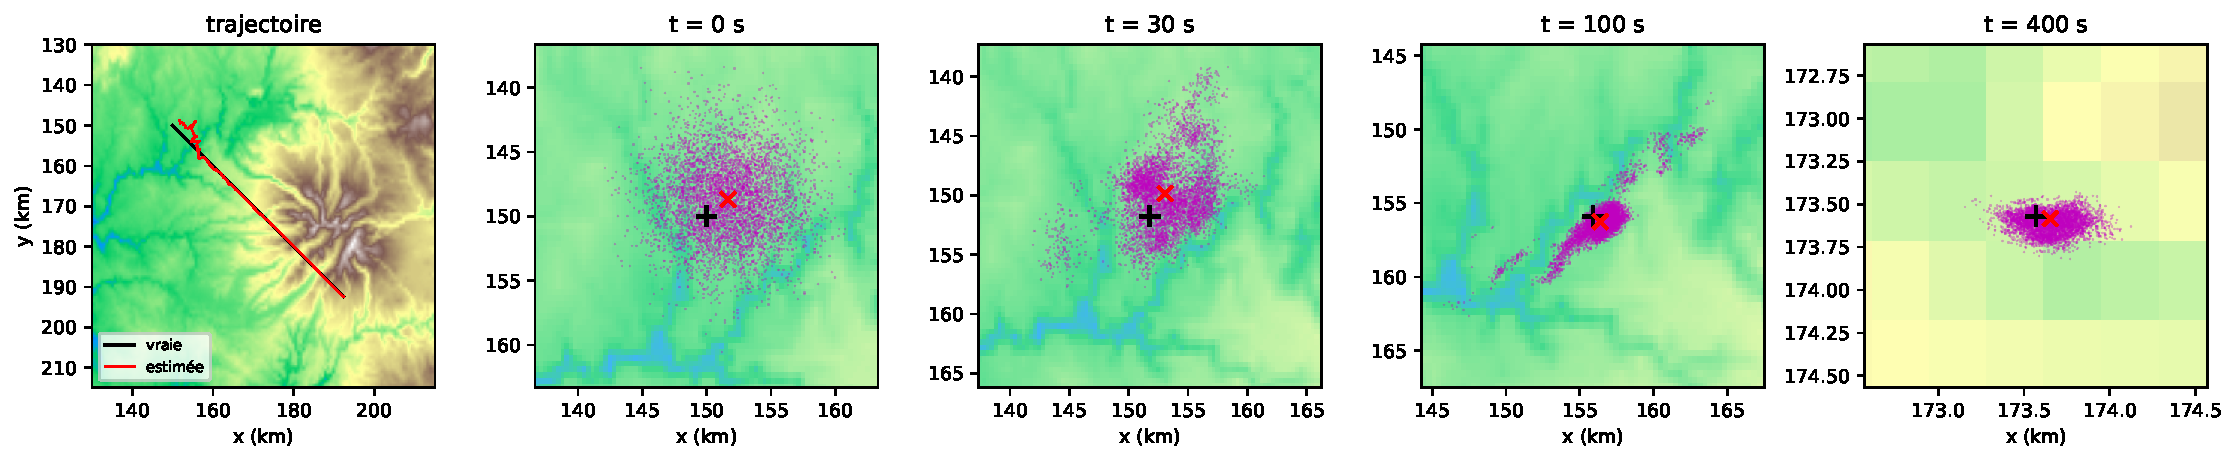
\includegraphics[width=\textwidth]{f1_carte_nuages.pdf}
\caption{Trajectoire vraie et estimée sur le MNT, puis nuage de particules à quatre
instants (croix noire : position vraie ; croix rouge : estimée). L'échelle des vignettes
se resserre avec le nuage.}\label{fig:carte}
\end{figure}

La figure~\ref{fig:carte} montre l'évolution du nuage. À $t=0$ il s'étend sur une
vingtaine de kilomètres et son centre est à $2{,}1$~km de la position vraie. À
$t=30$~s il s'est fragmenté en plusieurs paquets : la loi a posteriori est bien
multimodale. À $t=100$~s un mode principal contient la position vraie, mais des
paquets secondaires subsistent le long d'une bande. À $t=400$~s le nuage est unimodal
et large de quelques centaines de mètres, soit moins d'une maille de la carte.

\begin{figure}[H]
\centering
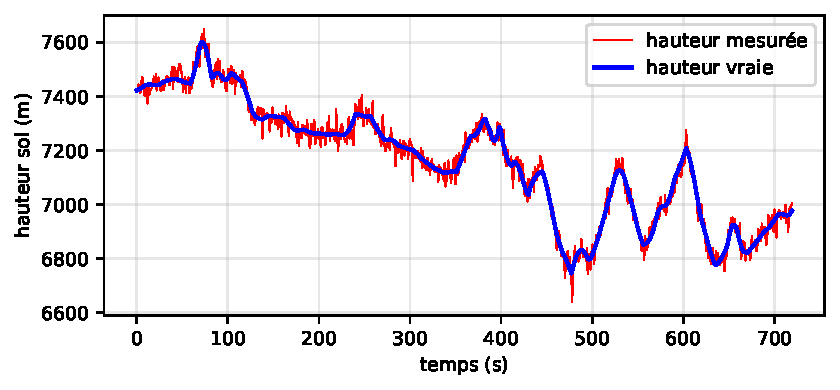
\includegraphics[width=0.49\textwidth]{f2_mesures.pdf}\hfill
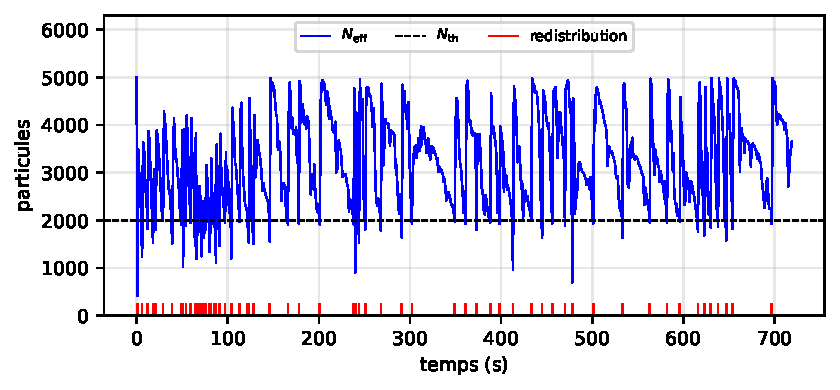
\includegraphics[width=0.49\textwidth]{f4_neff.pdf}
\caption{À gauche : hauteur sol vraie et mesurée. À droite : taille effective $\Neff$,
seuil $\Nth$ et instants de redistribution.}\label{fig:mesures}
\end{figure}

\begin{figure}[H]
\centering
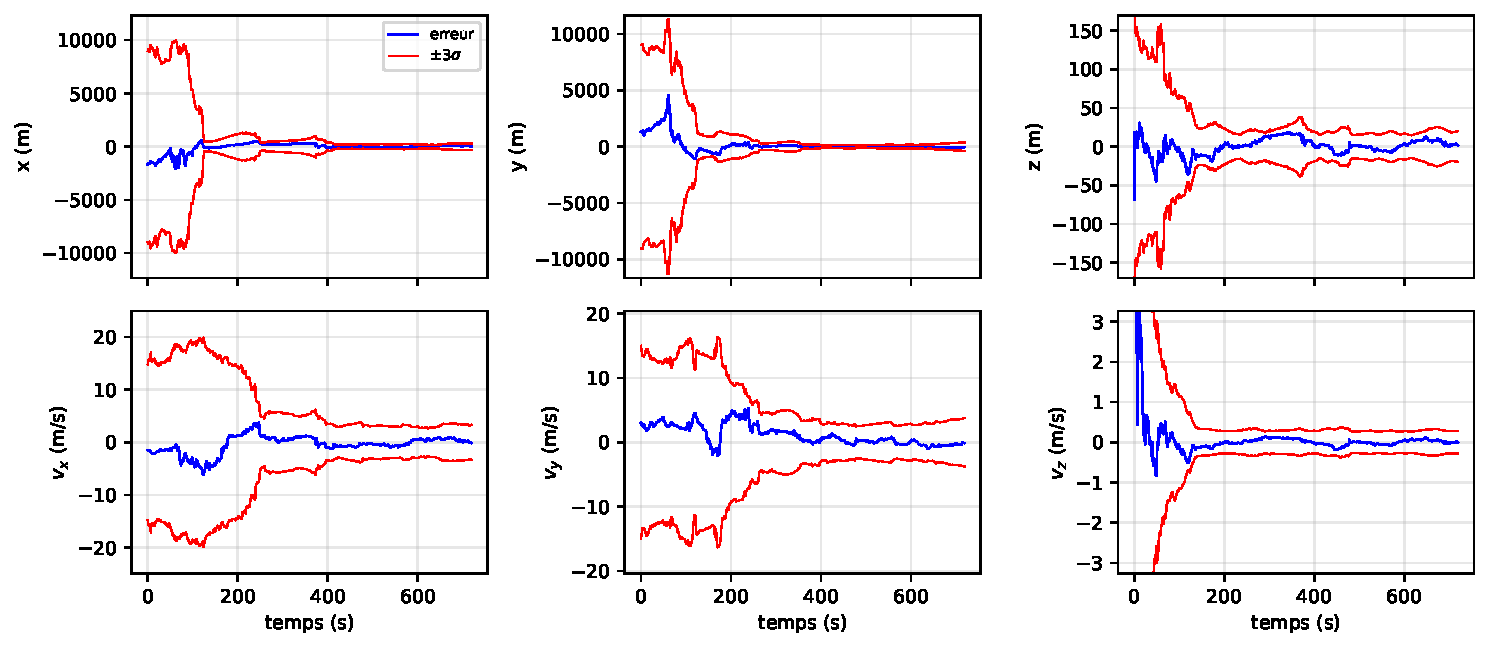
\includegraphics[width=\textwidth]{f3_erreurs.pdf}
\caption{Erreurs d'estimation (bleu) et enveloppes $\pm3\sigma$ tirées de $P_k$
(rouge), pour une réalisation.}\label{fig:erreurs}
\end{figure}

Sur cette réalisation, le filtre effectue $62$ redistributions, dont $23$ pendant les
$100$ premières secondes (figure~\ref{fig:mesures}, à droite) : c'est au début, quand
le nuage est large devant la vraisemblance, que les poids dégénèrent le plus vite. Les
erreurs (figure~\ref{fig:erreurs}) confirment l'analyse d'observabilité. L'altitude
converge en premier. Les enveloppes en $x$ et $y$ restent proches de $9$~km pendant
une centaine de secondes, puis s'effondrent entre $100$ et $150$~s, lorsque le relief
survolé a suffisamment varié. Les vitesses horizontales convergent en dernier, vers
$250$~s. En fin de vol l'erreur est de $22$~m en $x$, $-40$~m en $y$ et $1{,}5$~m en
$z$, et de moins de $0{,}15$~m/s sur chaque vitesse.

\subsection{Statistiques Monte-Carlo et cohérence}

Sur $50$ réalisations, aucune ne diverge (erreur horizontale finale supérieure à
$500$~m). En seconde moitié de vol, la médiane des erreurs quadratiques moyennes est
de $86$~m en horizontal, $5{,}1$~m en altitude et $0{,}5$~m/s sur les vitesses
horizontales. Le filtre effectue en moyenne $53$ redistributions par vol.

L'erreur vraie reste dans l'enveloppe $\pm3\sigma$ pendant plus de $99\,\%$ du temps
après $t=100$~s, pour chacune des six composantes. Le filtre n'est donc pas optimiste.
Il est même prudent : sur la réalisation de la figure~\ref{fig:erreurs}, les écarts-types
finaux en $x$ et $y$ ($102$ et $127$~m) dépassent les erreurs quadratiques observées
($87$ et $48$~m), ce qui est cohérent avec l'inflation de
covariance~\eqref{eq:inflation}.

\section{Étude de sensibilité}\label{sec:sensibilite}

Chaque configuration est évaluée sur $50$ réalisations. On reporte le taux de
divergence, et la médiane de l'erreur quadratique horizontale en seconde moitié de vol
calculée sur les seules réalisations convergées. Avec $50$ tirages, l'écart-type d'un
taux estimé peut atteindre $7$ points : seules les différences nettes sont
significatives.

\subsection{Nombre de particules}

\begin{figure}[H]
\centering
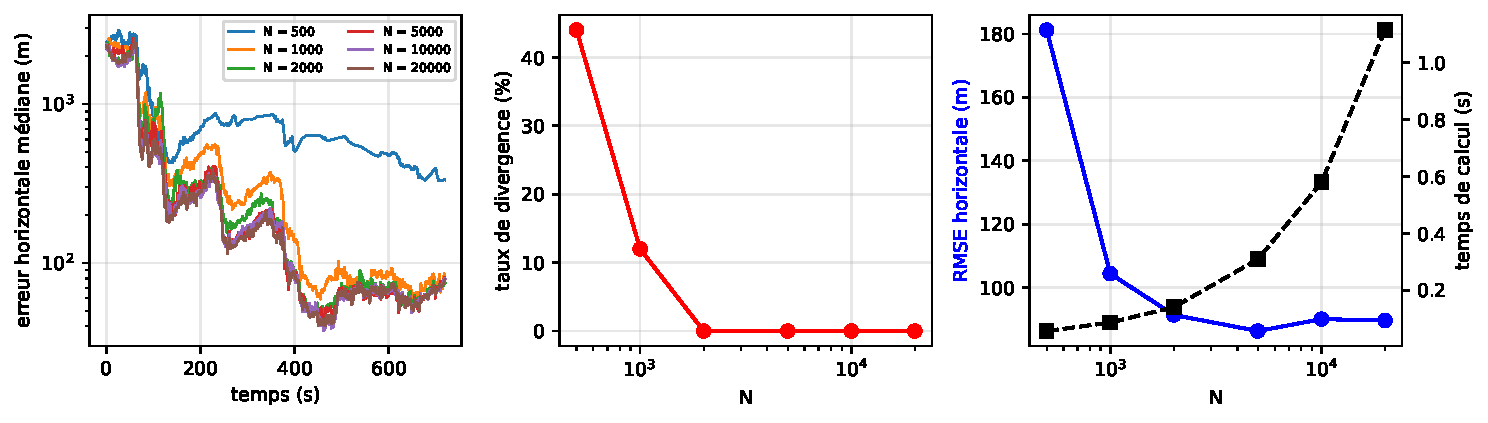
\includegraphics[width=\textwidth]{f5_nb_particules.pdf}
\caption{Influence de $N$ : erreur horizontale médiane au cours du temps, taux de
divergence, précision et temps de calcul d'un vol.}\label{fig:N}
\end{figure}

\begin{table}[H]
\centering\small
\begin{tabular}{rrrrrr}
\toprule
$N$ & divergence (\%) & erreur horiz. (m) & redistributions & $x$ dans $\pm3\sigma$ (\%) & temps (s)\\
\midrule
$500$ & 44 & 181 & 84 & 44 & 0,05\\
$1000$ & 12 & 104 & 62 & 81 & 0,08\\
$2000$ & 0 & 91 & 55 & 97 & 0,13\\
$5000$ & 0 & 86 & 53 & 100 & 0,28\\
$10000$ & 0 & 90 & 53 & 100 & 0,55\\
$20000$ & 0 & 90 & 52 & 100 & 1,10\\
\bottomrule
\end{tabular}
\caption{Influence du nombre de particules.}\label{tab:N}
\end{table}

Deux régimes apparaissent (figure~\ref{fig:N}, tableau~\ref{tab:N}). En dessous de
$2000$ particules, le nuage initial est trop clairsemé pour contenir des particules
proches de l'état vrai : le filtre diverge souvent ($44\,\%$ pour $N=500$) et devient
optimiste. À partir de $2000$ particules il ne diverge plus, et la précision plafonne
vers $90$~m : elle est alors limitée par l'information contenue dans les mesures
(bruit de $30$~m, pentes du relief), et non par l'erreur de Monte-Carlo. Le coût est
linéaire en $N$. La valeur $N=5000$ de l'énoncé offre donc une marge d'un facteur
$2{,}5$ sur le seuil de divergence pour $0{,}28$~s de calcul par vol de $720$~s.

\subsection{Pas de régularisation et noyau}

\begin{figure}[H]
\centering
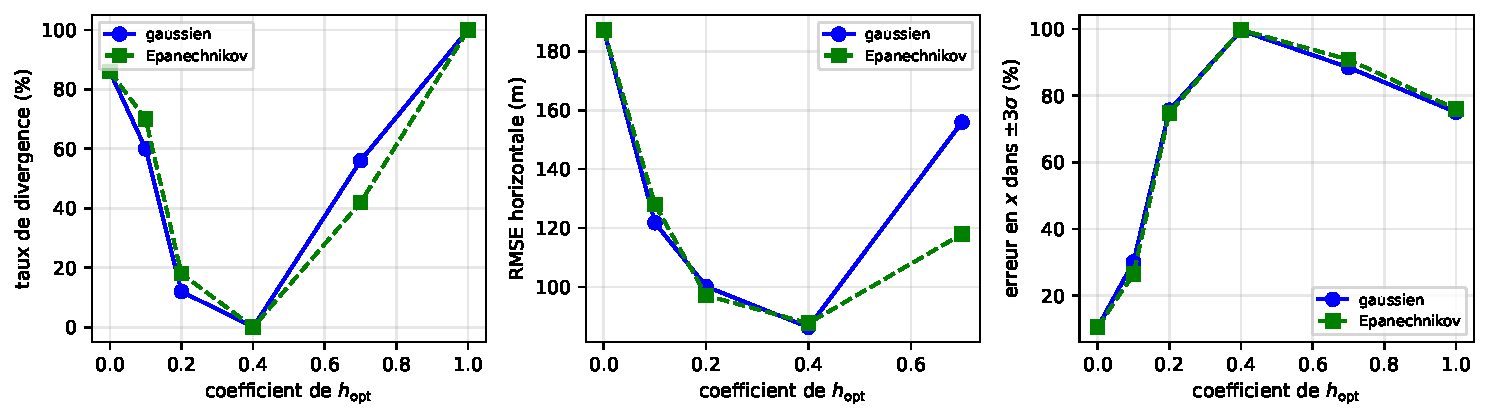
\includegraphics[width=\textwidth]{f6_regularisation.pdf}
\caption{Influence du coefficient appliqué à $\hopt$, pour les deux noyaux. Le
coefficient $0$ correspond au filtre SIR. Pour le coefficient $1$, aucune réalisation
ne converge.}\label{fig:h}
\end{figure}

C'est le paramètre le plus sensible (figure~\ref{fig:h}). La courbe du taux de
divergence a une forme en~U très marquée :
\begin{itemize}[nosep]
\item sans régularisation (SIR), le filtre diverge dans $86\,\%$ des cas et l'erreur en
$x$ n'est dans l'enveloppe $\pm3\sigma$ que $10\,\%$ du temps : le nuage s'effondre sur
quelques copies et le filtre est sûr de lui à tort ;
\item avec un coefficient de $0{,}1$ ou $0{,}2$, la diversité est encore insuffisante
($60\,\%$ puis $12\,\%$ de divergence avec le noyau gaussien) ;
\item avec $0{,}4$, aucune divergence ;
\item avec $0{,}7$ le filtre diverge dans $56\,\%$ des cas, et avec le pas optimal non
réduit dans $100\,\%$ des cas.
\end{itemize}
Ce dernier résultat s'explique par~\eqref{eq:inflation}. Avec $h=\hopt$, chaque
redistribution augmente la variance du nuage de $16\,\%$. Un nuage plus large rend la
vraisemblance plus piquée relativement au nuage, donc $\Neff$ chute plus vite, donc on
redistribue plus souvent : on compte $267$ redistributions par vol en moyenne, contre
$53$ avec le coefficient $0{,}4$. L'inflation s'emballe et le nuage quitte la zone
utile. La formule de $\hopt$ est optimale pour estimer une densité à un instant
donné, non pour une opération répétée des dizaines de fois.

Les deux noyaux donnent des résultats indiscernables à ce niveau de précision
statistique ($86$ et $88$~m au coefficient $0{,}4$). L'optimalité théorique du noyau
d'Epanechnikov n'a pas d'effet visible, ce qui est attendu puisque, d'après la
proposition~\ref{prop:tirage}, les deux noyaux injectent presque la même dispersion.
Le noyau gaussien, plus simple à tirer, suffit.

\subsection{Bruit d'état : SIR contre RPF}

\begin{figure}[H]
\centering
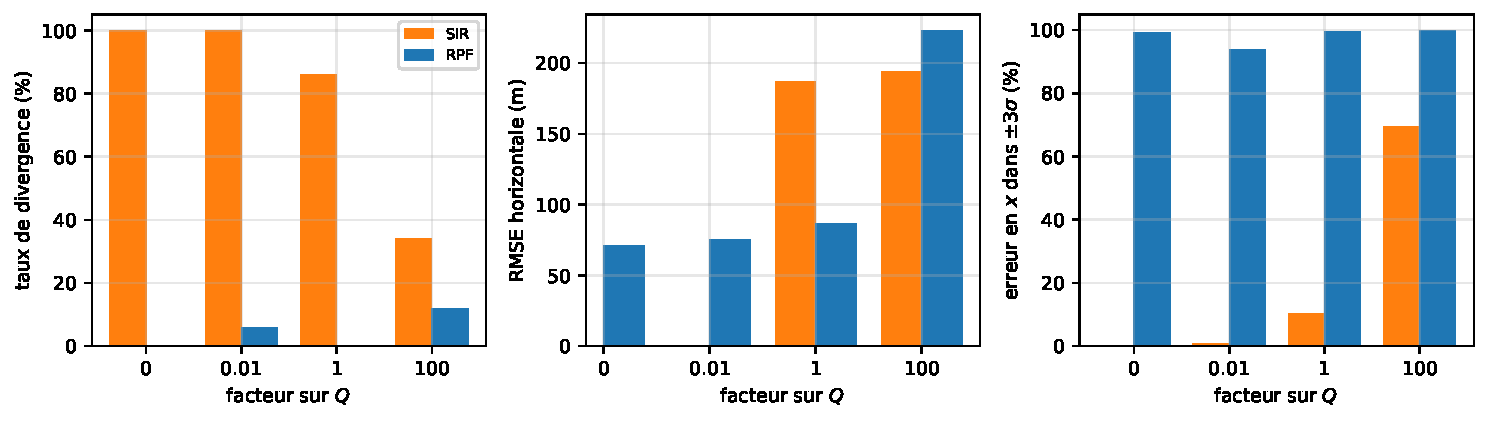
\includegraphics[width=\textwidth]{f7_bruit_etat.pdf}
\caption{Filtres SIR et RPF lorsque la covariance $Q$ du bruit d'état du filtre est
multipliée par $0$, $0{,}01$, $1$ et $100$. Barre absente : aucune réalisation
convergée.}\label{fig:Q}
\end{figure}

La figure~\ref{fig:Q} isole le rôle de la régularisation. Avec $Q=0$, le filtre SIR
diverge toujours : rien ne sépare les copies, et il ne reste en fin de vol que
$2$ particules distinctes (en médiane) sur $5000$. Le filtre RPF, lui, converge dans
tous les cas, et il est même plus précis qu'avec le $Q$ nominal ($71$~m contre $86$~m),
car la trajectoire vraie est ici sans bruit : le modèle $Q=0$ est le modèle exact. La
régularisation tient donc lieu de bruit d'état, avec l'avantage de s'adapter à la
taille du nuage au lieu d'être fixée à l'avance.

Quand $Q$ augmente, l'écart se réduit. Avec $Q\times100$, le bruit d'état apporte à
lui seul de la diversité et le filtre SIR ne diverge plus que dans $34\,\%$ des cas
(contre $12\,\%$ pour RPF), mais la précision des deux filtres se dégrade (environ
$200$~m) car le modèle de dynamique est devenu trop lâche. On retrouve la conclusion
du cours : la régularisation est surtout utile lorsque le bruit de dynamique est
faible.

\subsection{Seuil de redistribution, bruit de mesure, incertitude initiale}

\begin{table}[H]
\centering\small
\begin{tabular}{lrrr@{\hskip 3em}lrrr}
\toprule
\texttt{CoefResampling} & div. (\%) & err. (m) & redistr. &
$\sigma$ vrai (m) & div. (\%) & err. (m) & redistr.\\
\midrule
0,1 & 0 & 93 & 20 & 5 & 16 & 24 & 154\\
0,2 & 0 & 85 & 30 & 15 & 0 & 53 & 72\\
0,4 & 0 & 86 & 53 & 30 & 0 & 86 & 53\\
0,6 & 0 & 100 & 103 & 60 & 2 & 182 & 43\\
0,8 & 30 & 134 & 317 & 100 & 6 & 294 & 36\\
1,0 & 94 & 221 & 719 & & & &\\
\midrule
$\sigma_{\text{filtre}}/\sigma_{\text{vrai}}$ & div. (\%) & err. (m) & redistr. &
$\sigma_{xy}$ initial (m) & div. (\%) & err. (m) & redistr.\\
\midrule
0,5 & 88 & 137 & 269 & 1000 & 0 & 81 & 44\\
1,0 & 0 & 86 & 53 & 3000 & 0 & 86 & 53\\
1,5 & 0 & 80 & 34 & 6000 & 28 & 119 & 110\\
3,0 & 0 & 91 & 22 & 10000 & 86 & 450 & 172\\
\bottomrule
\end{tabular}
\caption{Taux de divergence, erreur horizontale médiane (réalisations convergées) et
nombre moyen de redistributions par vol, en faisant varier un seul paramètre à la
fois autour de la référence.}\label{tab:autres}
\end{table}

\paragraph{Seuil de redistribution.} Entre $0{,}1$ et $0{,}6$ le filtre est peu
sensible au seuil. Au-delà il se dégrade brutalement : redistribuer à chaque pas
(coefficient $1$) conduit à $94\,\%$ de divergence. C'est le même mécanisme de
sur-lissage que pour un grand $h$, puisque c'est le produit des facteurs
$1+h^2\sigma_K^2$ qui compte. Le seuil et le pas ne se règlent donc pas
indépendamment.

\paragraph{Bruit de mesure.} La précision suit le bruit de mesure, de $24$~m pour
$\sigma=5$~m à $294$~m pour $\sigma=100$~m. Mais des mesures très précises fragilisent
le filtre : avec $\sigma=5$~m la vraisemblance est si étroite que peu de particules
la recouvrent, on redistribue trois fois plus souvent et $16\,\%$ des vols divergent.
C'est le cas « peu de recouvrement entre densité prédite et vraisemblance » signalé
dans le cours.

\paragraph{Erreur sur le bruit de mesure.} Sous-estimer $\sigma$ dans le filtre est
catastrophique ($88\,\%$ de divergence avec un facteur $0{,}5$) : le filtre élimine
des particules correctes sur la foi de mesures qu'il croit trop précises.
Le surestimer est sans danger : avec un facteur $1{,}5$ ou $3$, aucune divergence, une
précision équivalente et moins de redistributions ($34$ et $22$ par vol contre $53$). Cela justifie le choix
du script fourni de gonfler $\sigma$ d'un facteur $1{,}5$.

\paragraph{Incertitude initiale.} À $N$ fixé, le filtre supporte $3$~km mais pas
$6$~km ($28\,\%$ de divergence) ni $10$~km ($86\,\%$). La densité surfacique de
particules décroît comme $1/\sigma_{xy}^2$ : passer de $3$ à $10$~km la divise par
$11$, ce qui ramène dans le régime clairsemé observé pour $N=500$.

\subsection{Limites}

Notre étude a trois limites. D'une part, les mesures sont simulées avec la même carte
et la même interpolation que celles du filtre : les erreurs de carte, qui existent en
pratique, ne sont pas représentées. D'autre part, nous n'avons étudié qu'une
trajectoire, au-dessus d'un relief marqué ; d'après la section~\ref{sec:modele}, un
survol de terrain plat devrait ralentir la convergence, ce que nous n'avons pas
vérifié numériquement. Enfin, la moyenne pondérée est un mauvais estimateur tant que
plusieurs modes coexistent (figure~\ref{fig:carte}, $t=30$~s) : elle peut tomber entre
deux modes, là où il n'y a aucune particule.

\section{Conclusion}

Le recalage altimétrique est un problème où la mesure est une table de relief et
où la loi a posteriori commence par être multimodale ; le filtre particulaire le
traite sans linéarisation. Avec les réglages de l'énoncé, le filtre régularisé
converge dans toutes nos réalisations, ramène une incertitude de $3$~km à moins de
$100$~m d'erreur horizontale et quelques mètres en altitude, et reste cohérent avec
sa propre covariance.

Le résultat principal de l'étude de sensibilité concerne la régularisation. Elle est
indispensable, parce que le bruit d'état est trop faible pour redonner de la
diversité au nuage : le filtre SIR diverge dans $86\,\%$ des cas. Mais elle gonfle la
covariance d'un facteur $1+h^2\sigma_K^2$ à chaque redistribution, de sorte que le
pas optimal de l'estimation de densité, appliqué tel quel, fait diverger le filtre à
coup sûr. Le coefficient $0{,}4$ de l'énoncé se situe au creux de ce compromis. Les
autres enseignements sont qu'il faut au moins $2000$ particules pour $3$~km
d'incertitude initiale, que le choix du noyau importe peu, et qu'il vaut mieux
surestimer le bruit de mesure que le sous-estimer.

\begin{thebibliography}{9}\small
\bibitem{dahia} K.~Dahia, \emph{Filtrage bayésien et navigation, TP4 : filtrage
particulaire}, support de cours, ENSTA, 2026.
\bibitem{gordon} N.~J.~Gordon, D.~J.~Salmond, A.~F.~M.~Smith, Novel approach to
nonlinear/non-Gaussian Bayesian state estimation, \emph{IEE Proceedings F}
\textbf{140} (1993), 107--113.
\bibitem{kong} A.~Kong, J.~S.~Liu, W.~H.~Wong, Sequential imputations and Bayesian
missing data problems, \emph{J.\ Amer.\ Statist.\ Assoc.}\ \textbf{89} (1994), 278--288.
\bibitem{musso} C.~Musso, N.~Oudjane, F.~Le~Gland, Improving regularised particle
filters, in \emph{Sequential Monte Carlo Methods in Practice}, A.~Doucet,
N.~de~Freitas, N.~Gordon (éd.), Springer, 2001, 247--271.
\bibitem{silverman} B.~W.~Silverman, \emph{Density Estimation for Statistics and Data
Analysis}, Chapman \& Hall, 1986.
\bibitem{arulampalam} M.~S.~Arulampalam, S.~Maskell, N.~Gordon, T.~Clapp, A tutorial
on particle filters for online nonlinear/non-Gaussian Bayesian tracking,
\emph{IEEE Trans.\ Signal Process.}\ \textbf{50} (2002), 174--188.
\end{thebibliography}

\end{document}
